\documentclass[11pt,a4paper]{article}

\usepackage[utf8]{inputenc}
\usepackage[T1]{fontenc}
\usepackage[spanish]{babel}
\usepackage{amsmath}
\usepackage{amsfonts}
\usepackage{amssymb}
\usepackage{graphicx}
\usepackage{tabularx}
\usepackage{booktabs}
\usepackage{hyperref}
\usepackage{geometry}
\usepackage{listings}
\usepackage{xcolor}
\usepackage{caption}
\usepackage{subcaption}
\usepackage{titlesec}
\usepackage{parskip}
\usepackage{float}

% Configuración de títulos de párrafos
\titleformat{\paragraph}[hang]
{\normalfont\normalsize\bfseries}{\theparagraph}{1em}{}
\titlespacing*{\paragraph}
{0pt}{3.25ex plus 1ex minus .2ex}{1em}

\geometry{top=3cm, bottom=3cm, left=2.5cm, right=2.5cm}

\hypersetup{
    colorlinks=true,
    linkcolor=black,
    filecolor=magenta,      
    urlcolor=cyan,
}

\definecolor{codegreen}{rgb}{0,0.6,0}
\definecolor{codegray}{rgb}{0.5,0.5,0.5}
\definecolor{codepurple}{rgb}{0.58,0,0.82}
\definecolor{backcolour}{rgb}{0.95,0.95,0.92}

\lstdefinestyle{mystyle}{
    backgroundcolor=\color{backcolour},   
    commentstyle=\color{codegreen},
    keywordstyle=\color{magenta},
    numberstyle=\tiny\color{codegray},
    stringstyle=\color{codepurple},
    basicstyle=\ttfamily\small,
    breakatwhitespace=false,         
    breaklines=true,                 
    captionpos=b,                    
    keepspaces=true,                 
    numbers=left,                    
    numbersep=5pt,                  
    showspaces=false,                
    showstringspaces=false,
    showtabs=false,                  
    tabsize=2
}

\lstset{style=mystyle}

\begin{document}
\begin{titlepage}
    \begin{center}
        \vspace*{1cm}

        \Huge
        \textbf{Trabajo Practico N°3}

        \vspace{0.5cm}
        \LARGE
        Fixed Point

        \vspace{1.5cm}

        \vfill

        \Large
        \textbf{Autor:} Simón Saillen

        \Large
        \textbf{Profesores:} Ariel Luis Pola, Agustin Pesce, Pablo Cayuela, Paul Romero, Santiago Garaventta Pascual

        \vspace{0.5cm}

        \Large
        \textbf{Fundación Fulgor}\\
        Julio 2026

    \end{center}
\end{titlepage}
\newpage

\section{Introducción}

En el Procesamiento Digital de Señales (DSP), los cálculos en punto flotante
ofrecen alta precisión pero requieren recursos significativos de hardware. La
aritmética de punto fijo permite reducir la complejidad del hardware a costa de
una pérdida controlada de precisión.

Este trabajo práctico aborda el impacto de la cuantización de coeficientes de
un filtro de caída cosenoidal (raised cosine) utilizado en comunicaciones
digitales. Se parte de un simulador en punto flotante desarrollado en Python y
se aplican distintas configuraciones de punto fijo sobre los coeficientes del
filtro, observando cómo afectan la respuesta al impulso, la respuesta en
frecuencia, la convolución con los símbolos transmitidos y la constelación
resultante.

\section{Objetivos}

\begin{itemize}
    \item Generar tres filtros de caída cosenoidal con factores de roll-off $\beta =
              [0.0;\ 0.5;\ 1.0]$ en punto flotante, con $N_{baud} = 16$, $F_{baud} = 1$\,GHz
          y sobremuestreo $OS = 8$.
    \item Graficar la respuesta al impulso y la respuesta en frecuencia de cada filtro.
    \item Convolucionar los filtros con símbolos aleatorios $\pm 1$ y graficar la
          constelación resultante con fase óptima.
    \item Aplicar sobre cada filtro las cuantizaciones $S(8,7)$, $S(6,4)$ y $S(3,2)$ en
          modos \texttt{trunc} y \texttt{round}, siempre con saturación.
\end{itemize}

\section{Desarrollo}

\subsection{Simulador en punto flotante}

Se desarrolló el script \texttt{fixedPoint.py}, inspirado en el script brindado
\texttt{tx\_rcosine\_procom.py}, que implementa el modelo de un sistema de
comunicaciones con filtrado de caída cosenoidal. Los parámetros utilizados
fueron:

\begin{itemize}
    \item Período de baudio: $T = 1$\,ns ($F_{baud} = 1$\,GHz)
    \item Símbolos: $N_{symb} = 1000$
    \item Sobremuestreo: $OS = 8$
    \item Longitud del filtro: $N_{baud} = 16$ símbolos
    \item Roll-off: $\beta \in \{0.0;\ 0.5;\ 1.0\}$
\end{itemize}

Para la generación de los filtros se utilizó la función \texttt{rcosine()} de
\texttt{DSPtools.py}, que implementa la respuesta al impulso del pulso de caída
cosenoidal.

Se generaron símbolos aleatorios binarios $\pm 1$ para las componentes I
(in-phase) y Q (quadrature), se insertaron $OS-1$ ceros entre símbolos
(upsampling) y se convolucionó con cada filtro.

Finalmente se downsampleó con fase óptima para obtener la constelación.

\subsection{Cuántización de coeficientes}

Para la cuantización se utilizó la clase \texttt{DeFixedInt} de la biblioteca
\texttt{\_fixedInt.py} (basada en \texttt{deModel} de Dillon Engineering),
modificada para soportar los modos de saturación, truncamiento y redondeo
requeridos. Se empleó la función \texttt{arrayFixedInt()} que recibe un array
de valores flotantes y devuelve un array de objetos \texttt{DeFixedInt} con la
representación de punto fijo deseada.

Las configuraciones aplicadas fueron:

\begin{itemize}
    \item $S(8,7)$: 8 bits totales, 7 fraccionales (rango $\approx \pm 1$,
          resolución $2^{-7} \approx 0.0078$)
    \item $S(6,4)$: 6 bits totales, 4 fraccionales (rango $\approx \pm 2$,
          resolución $2^{-4} = 0.0625$)
    \item $S(3,2)$: 3 bits totales, 2 fraccionales (rango $\approx \pm 1$,
          resolución $2^{-2} = 0.25$)
\end{itemize}

Cada configuración se aplicó en modo \texttt{trunc} (truncado) y \texttt{round}
(redondeo), siempre con saturación antidesborde (\texttt{saturate}),
totalizando 6 cuantizaciones por filtro.

\section{Resultados}

\subsection{Respuesta al impulso}

En la figura se muestra la respuesta al impulso de los tres filtros en punto
flotante. Puede observarse cómo el filtro con $\beta = 0.0$ (sinc puro)
presenta lóbulos laterales que decaen lentamente, mientras que $\beta = 1.0$
tiene colas mucho más suaves a costa de mayor ancho de banda.

\begin{figure}[H]
    \centering
    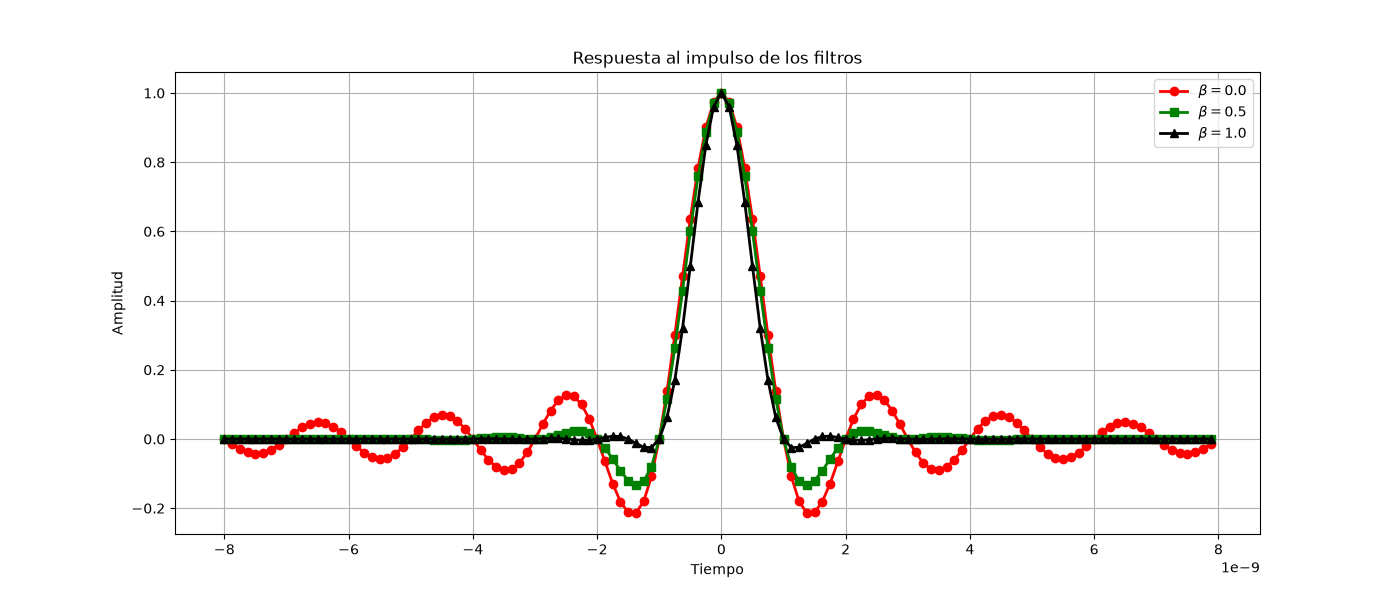
\includegraphics[width=0.85\textwidth]{../images/impulso.png}
    \caption{Respuesta al impulso de los filtros de caída cosenoidal en
        punto flotante.}
\end{figure}

Al cuantizar los coeficientes, los efectos son más notorios cuanto menor es la
cantidad de bits. En la siguientes figuras se comparan la respuesta al impulso
para $\beta = 0.5$ con las tres cuantizaciones en modo truncado y redondeado.
La cuantización $S(8,7)$ (amarillo) es prácticamente indistinguible del
original, $S(3,2)$ (verde) produce una distorsión notable en los lóbulos
laterales y $S(6,4)$ (azul) presenta pequeñas diferencias de la original.

\begin{figure}[H]
    \centering
    \begin{subfigure}[b]{0.49\textwidth}
        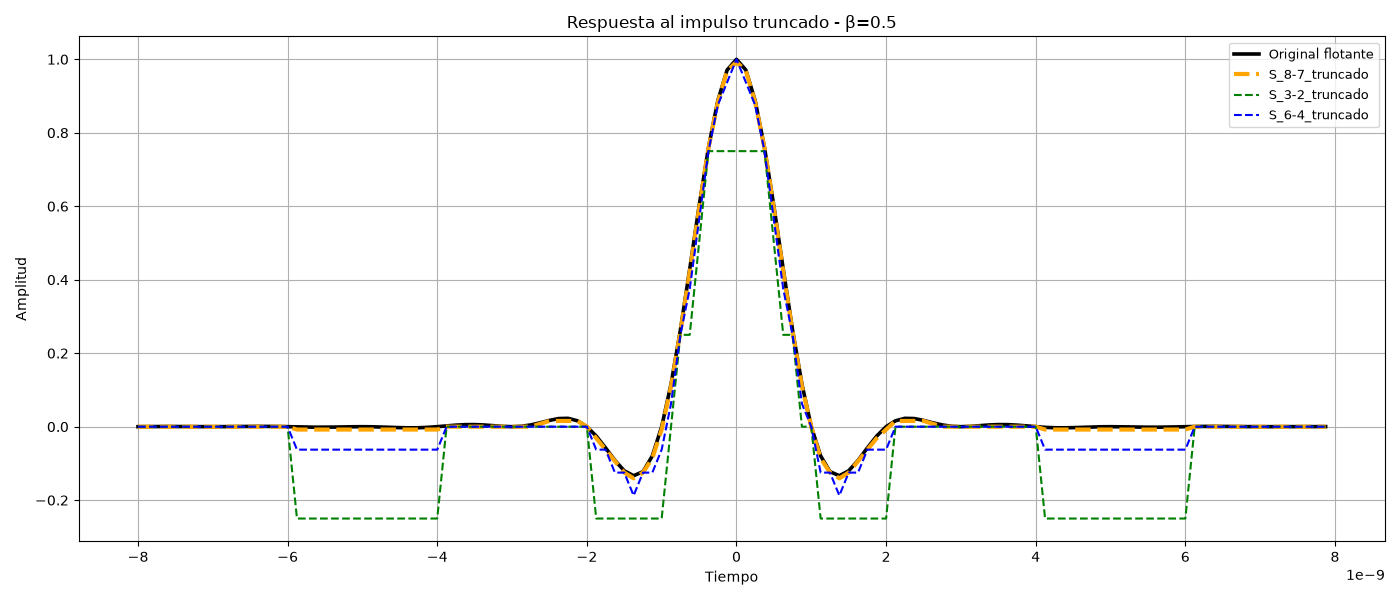
\includegraphics[width=\textwidth]{../images/cuantizaciones/impulso_truncado_beta1.png}
        \caption{Truncado, $\beta = 0.5$.}
    \end{subfigure}
    \hfill
    \begin{subfigure}[b]{0.49\textwidth}
        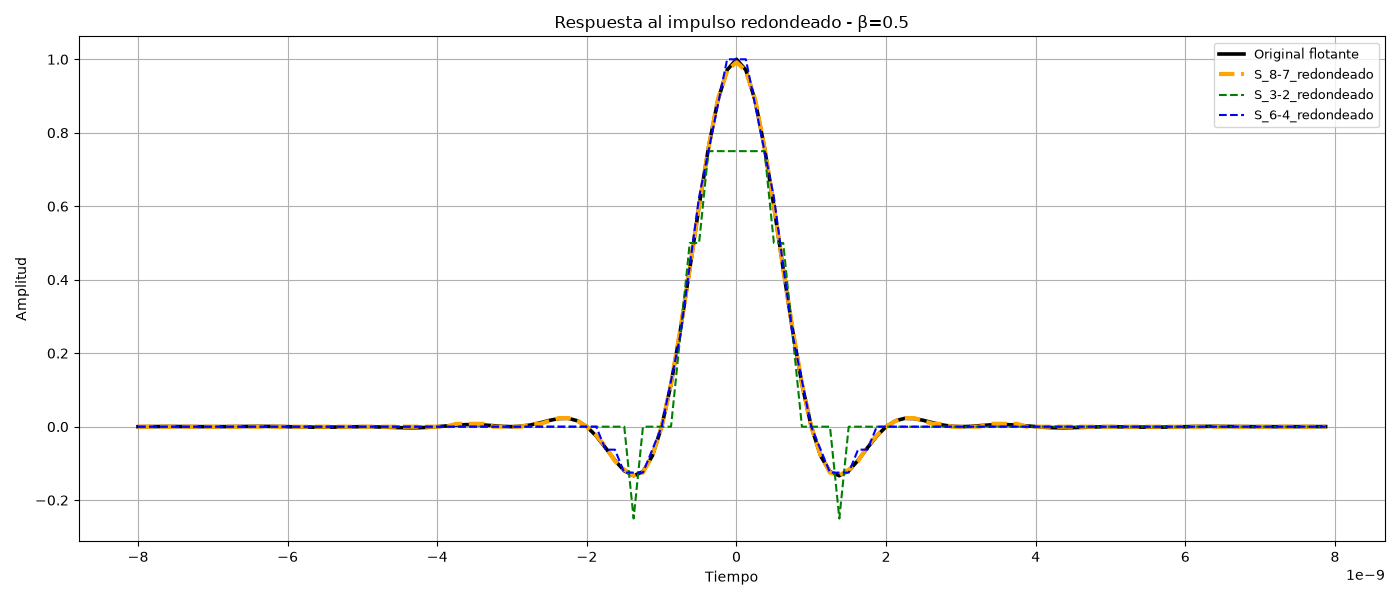
\includegraphics[width=\textwidth]{../images/cuantizaciones/impulso_redondeado_beta1.png}
        \caption{Redondeado, $\beta = 0.5$.}
    \end{subfigure}
    \caption{Respuestas al impulso cuantizadas --- Truncado y Redondeado}
\end{figure}

En las Figuras 3.a y 3.b se muestran los casos restantes para $\beta = 0.0$ y
$\beta = 1.0$ en modo truncado.

\begin{figure}[H]
    \centering
    \begin{subfigure}[b]{0.49\textwidth}
        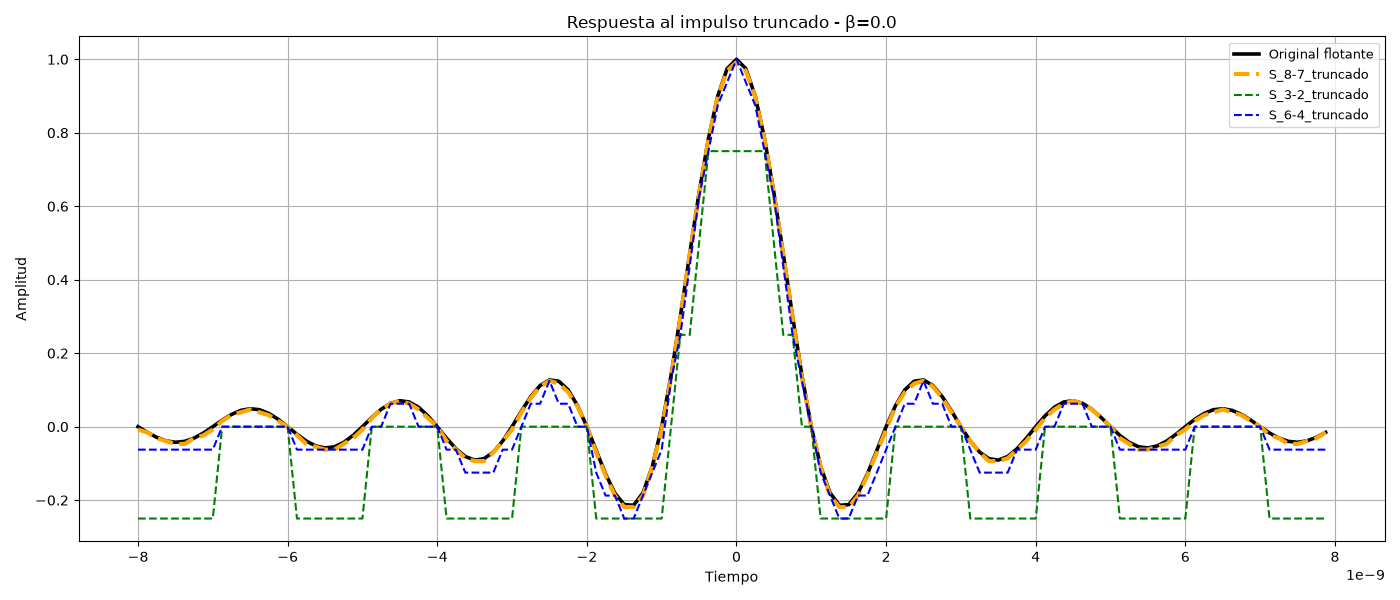
\includegraphics[width=\textwidth]{../images/cuantizaciones/impulso_truncado_beta0.png}
        \caption{Truncado, $\beta = 0.0$.}
    \end{subfigure}
    \hfill
    \begin{subfigure}[b]{0.49\textwidth}
        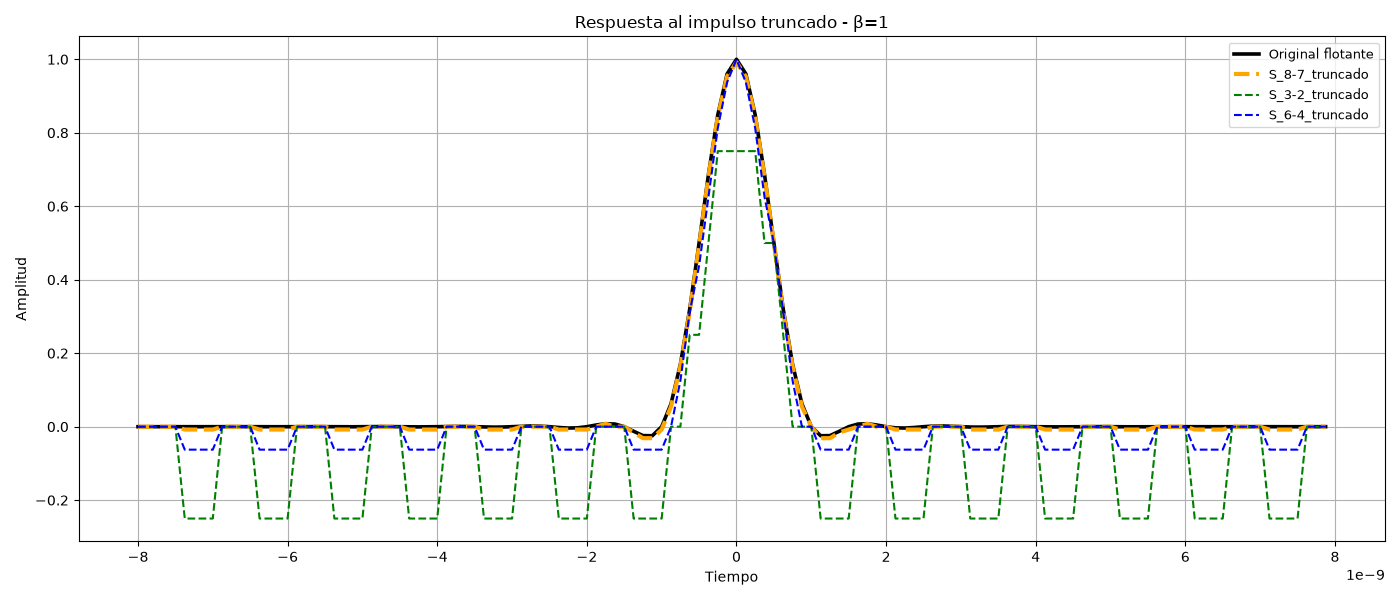
\includegraphics[width=\textwidth]{../images/cuantizaciones/impulso_truncado_beta2.png}
        \caption{Truncado, $\beta = 1.0$.}
    \end{subfigure}
    \caption{Respuesta al impulso cuantizada --- truncado.}
\end{figure}

En las Figuras 4.a y 4.b se muestran los casos restantes para $\beta = 0.0$ y
$\beta = 1.0$ en modo redondeado.

\begin{figure}[H]
    \centering
    \hfill
    \begin{subfigure}[b]{0.49\textwidth}
        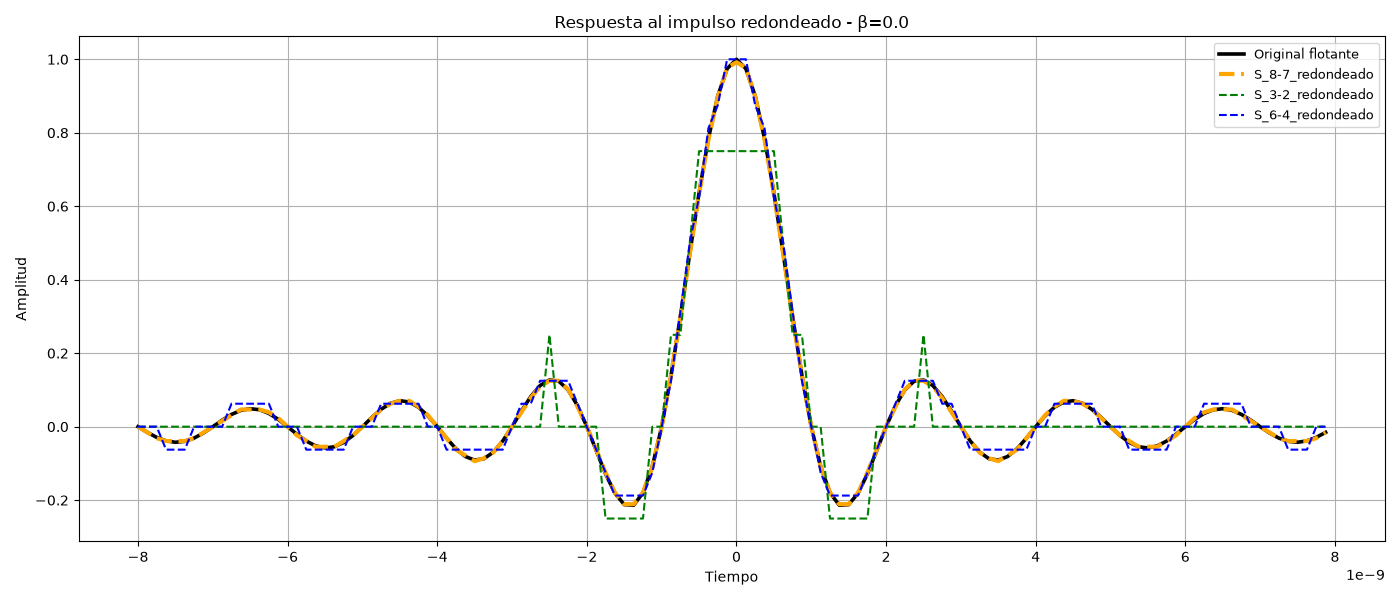
\includegraphics[width=\textwidth]{../images/cuantizaciones/impulso_redondeado_beta0.png}
        \caption{Redondeado, $\beta = 0.0$.}
    \end{subfigure}
    \hfill
    \begin{subfigure}[b]{0.49\textwidth}
        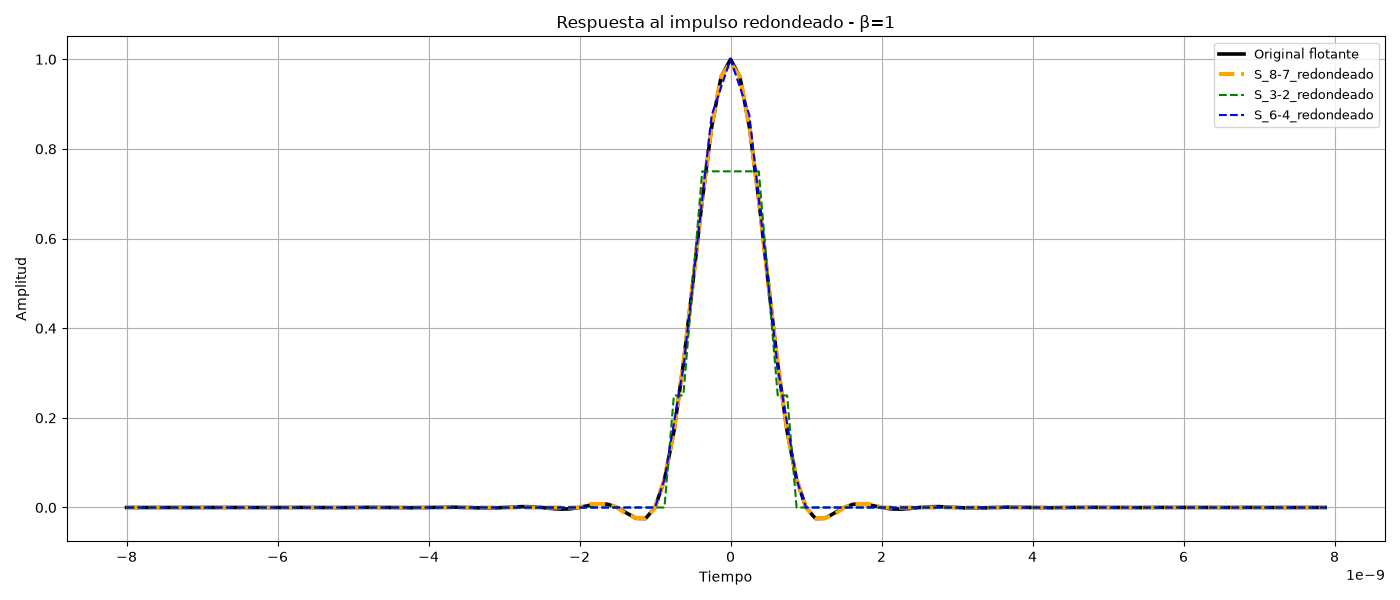
\includegraphics[width=\textwidth]{../images/cuantizaciones/impulso_redondeado_beta2.png}
        \caption{Redondeado, $\beta = 1.0$.}
    \end{subfigure}
    \caption{Respuesta al impulso cuantizada --- redondeado.}
\end{figure}

\subsection{Respuesta en frecuencia}

En la siguiente figura se muestra la respuesta en frecuencia de los tres
filtros en punto flotante. Puede observarse como el ancho de banda ocupado
aumenta conforme crece beta: $\beta = 0.0$ ocupa el mínimo ancho
($F_{baud}/2$), mientras que $\beta = 1.0$ duplica ese ancho. Como
consecuencia, la energía en la banda de transición es menor para $\beta = 0.0$
y mayor para $\beta = 1.0$, lo que se traduce en una caída más abrupta a costa
de una mayor sensibilidad al truncamiento temporal del filtro. También es
apreciable cómo el filtro $\beta = 0.0$ presenta un lóbulo secundario más
pronunciado en frecuencia debido a la naturaleza abrupta del corte, mientras
que $\beta = 1.0$ tiene una transición más suave.

\begin{figure}[H]
    \centering
    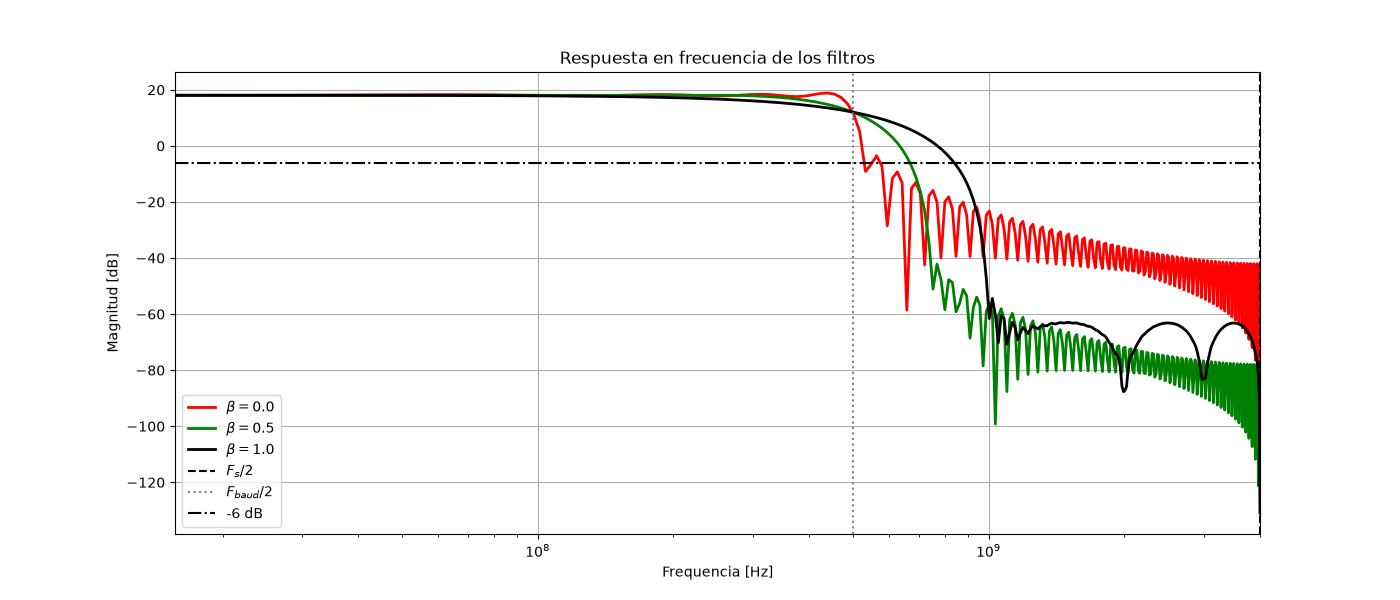
\includegraphics[width=0.85\textwidth]{../images/frecuencia.png}
    \caption{Respuesta en frecuencia de los filtros en punto flotante.}
\end{figure}

Al cuantizar, las diferencias se aprecian principalmente en la banda de
rechazo. La cuantización $S(3,2)$ (verde) eleva el piso de ruido espectral de
forma considerable, mientras que $S(8,7)$ (amarillo) preserva casi intacta la
respuesta original. En las figuras 6.a y 6.b se muestra el caso más crítico
($\beta = 0.0$, truncado y redondeado).

\begin{figure}[H]
    \centering
    \begin{subfigure}[b]{0.49\textwidth}
        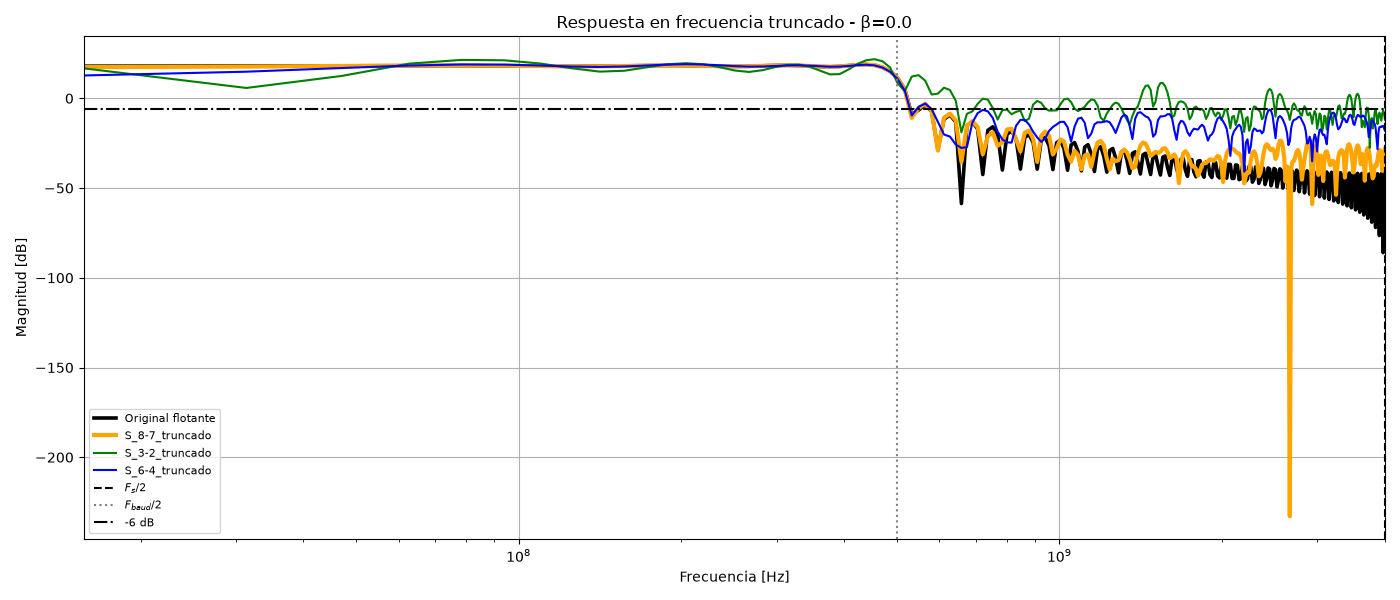
\includegraphics[width=\textwidth]{../images/cuantizaciones/frecuencia_truncado_beta0.png}
        \caption{Truncado, $\beta = 0.0$.}
    \end{subfigure}
    \hfill
    \begin{subfigure}[b]{0.49\textwidth}
        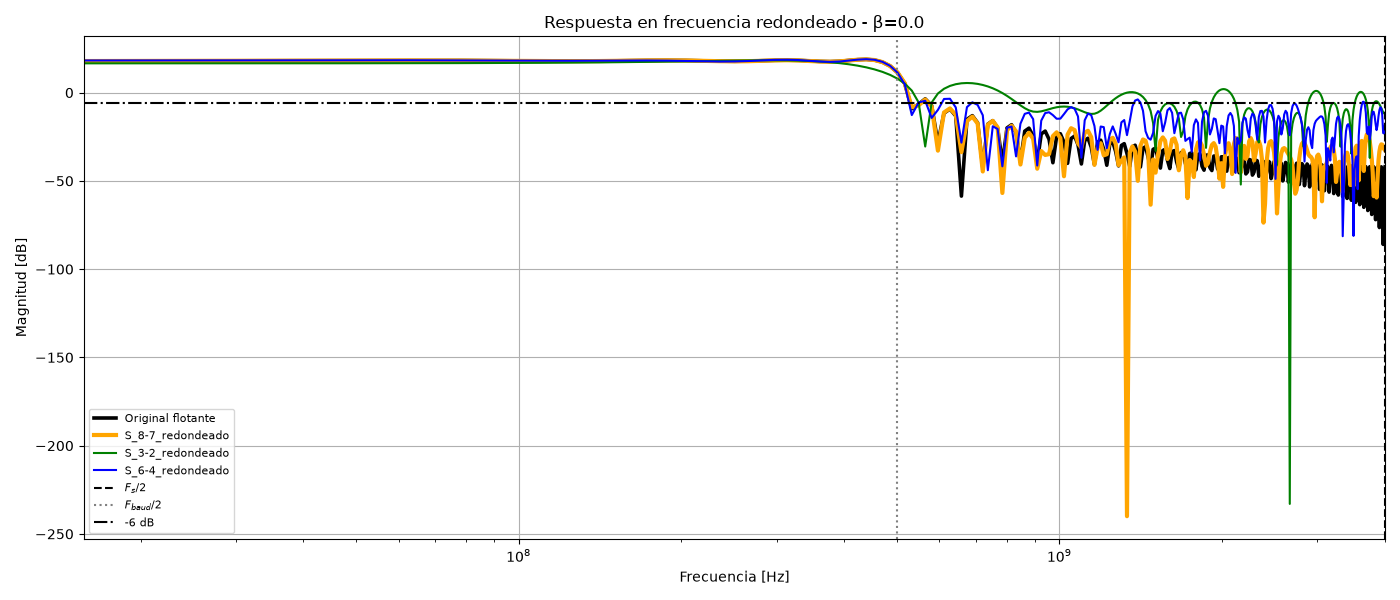
\includegraphics[width=\textwidth]{../images/cuantizaciones/frecuencia_redondeado_beta0.png}
        \caption{Redondeado, $\beta = 0.0$.}
    \end{subfigure}
    \caption{Respuesta en frecuencia cuantizada para $\beta = 0.0$.}
\end{figure}

Las Figuras 7.a y 7.b se muestran los resultados para $\beta = 0.5$ y $\beta =
    1.0$ con truncado, donde se observa cómo el filtro de mayor ancho de banda es
menos afectado por la cuantización.

\begin{figure}[H]
    \centering
    \begin{subfigure}[b]{0.49\textwidth}
        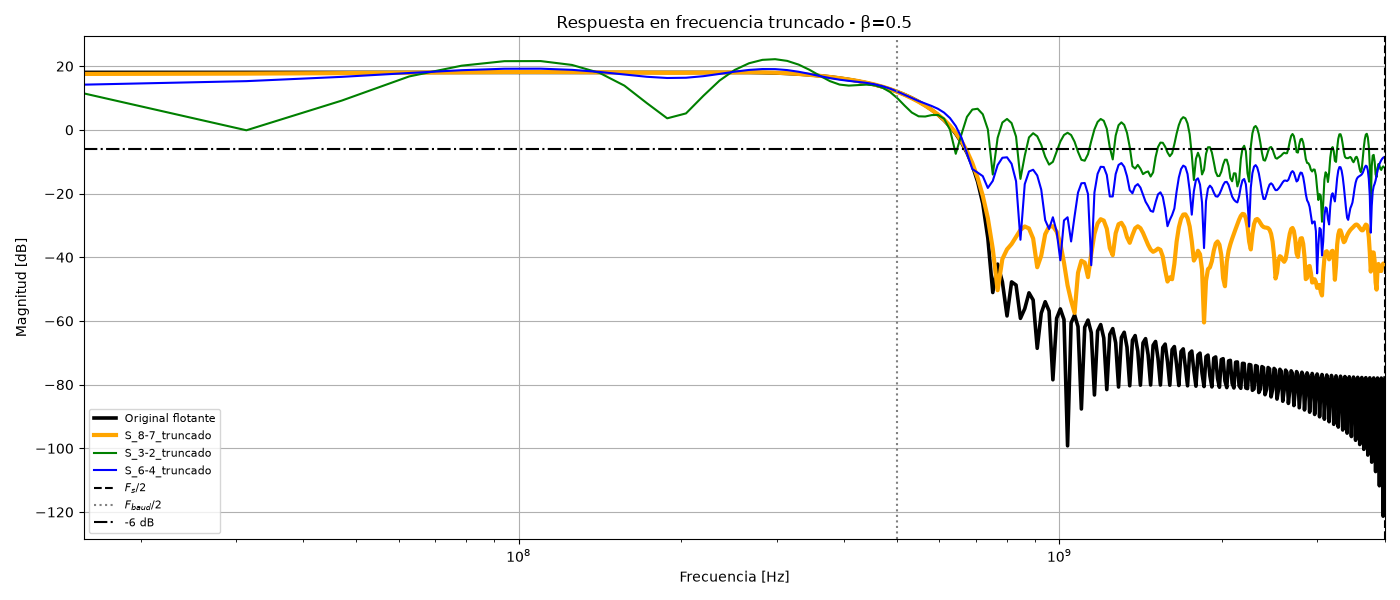
\includegraphics[width=\textwidth]{../images/cuantizaciones/frecuencia_truncado_beta1.png}
        \caption{Truncado, $\beta = 0.5$.}
    \end{subfigure}
    \hfill
    \begin{subfigure}[b]{0.49\textwidth}
        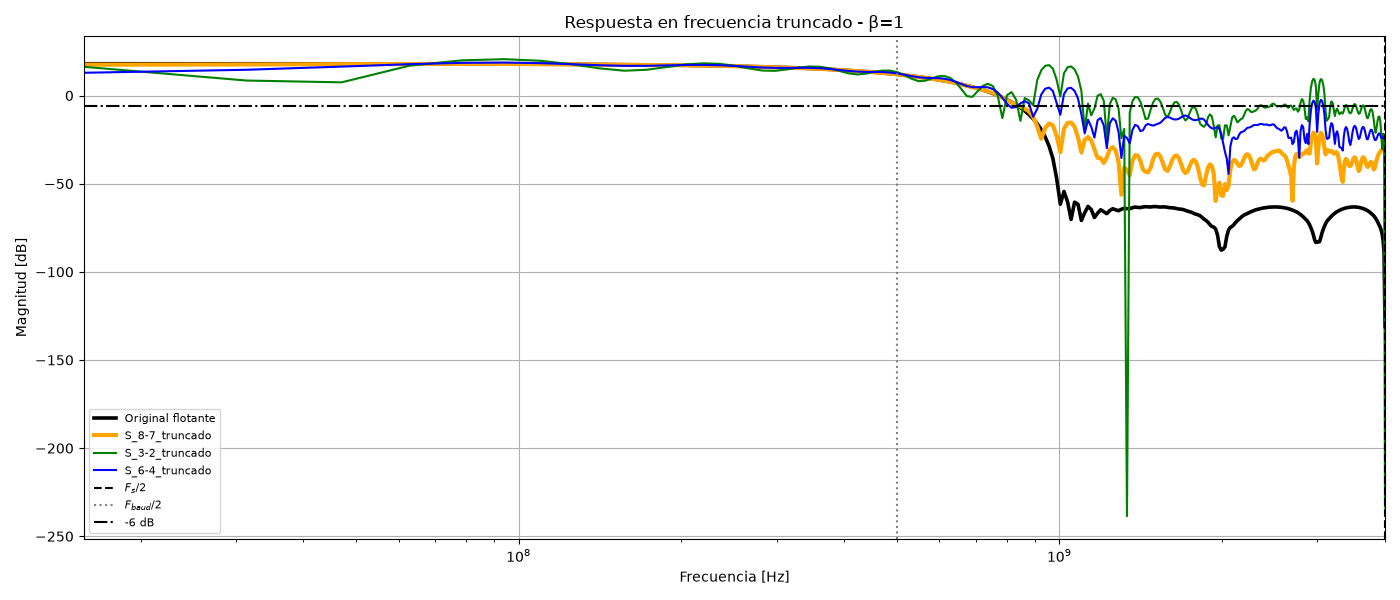
\includegraphics[width=\textwidth]{../images/cuantizaciones/frecuencia_truncado_beta2.png}
        \caption{Truncado, $\beta = 1.0$.}
    \end{subfigure}
    \caption{Respuesta en frecuencia cuantizada --- truncado.}
\end{figure}

Las Figuras 8.a y 8.b se muestran los resultados para $\beta = 0.5$ y $\beta =
    1.0$ con redondeado.

\begin{figure}[H]
    \centering
    \begin{subfigure}[b]{0.49\textwidth}
        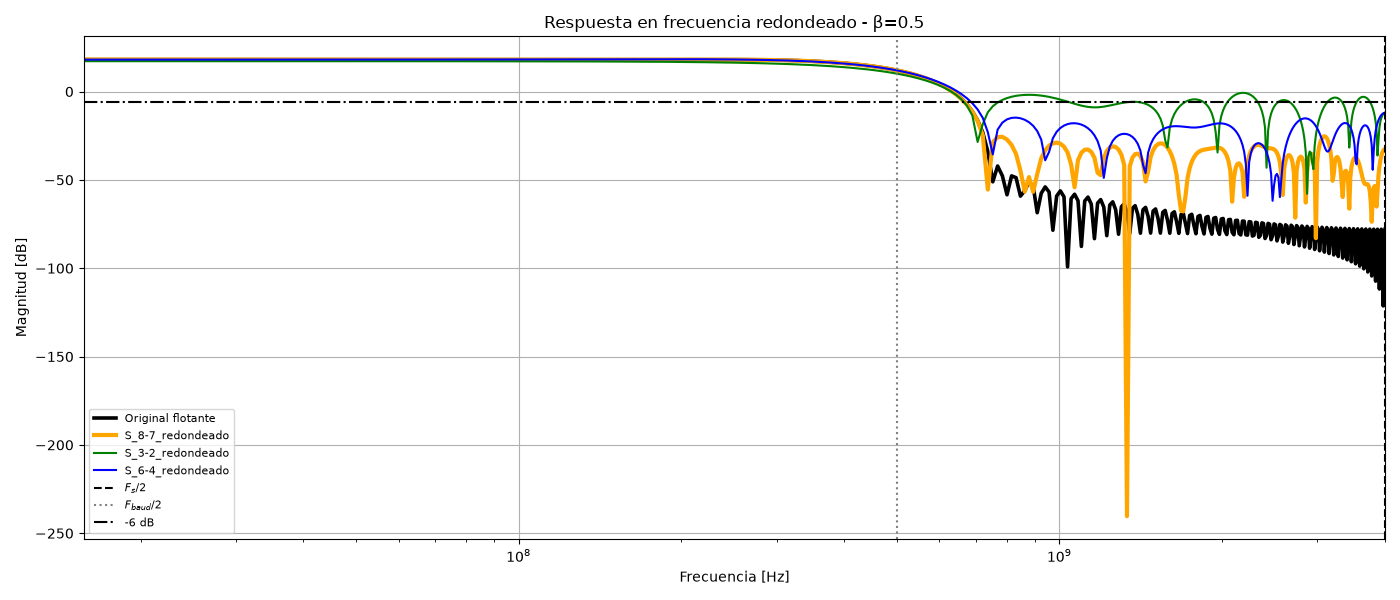
\includegraphics[width=\textwidth]{../images/cuantizaciones/frecuencia_redondeado_beta1.png}
        \caption{Redondeado, $\beta = 0.5$.}
    \end{subfigure}
    \hfill\begin{subfigure}[b]{0.49\textwidth}
        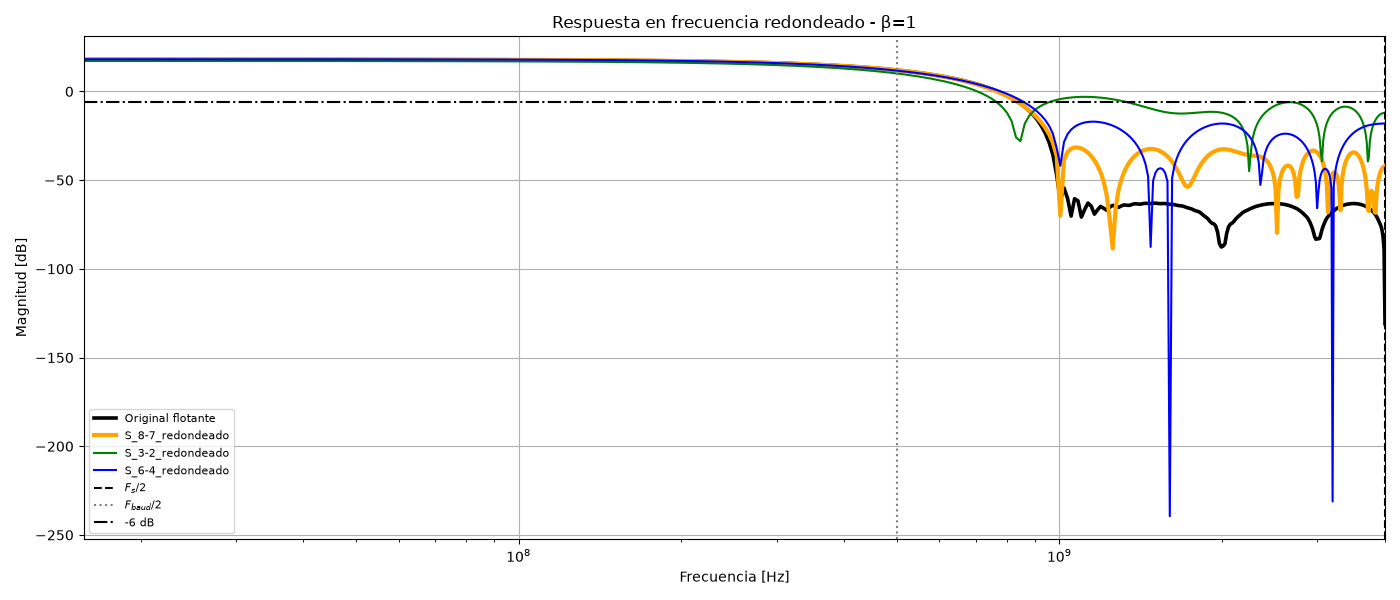
\includegraphics[width=\textwidth]{../images/cuantizaciones/frecuencia_redondeado_beta2.png}
        \caption{Redondeado, $\beta = 1.0$.}
    \end{subfigure}
    \caption{Respuesta en frecuencia cuantizada --- redondeado.}
\end{figure}

\subsection{Convolución con los símbolos}

La convolución de los filtros con los símbolos transmitidos (con ceros
intercalados) permite observar el efecto del filtrado en el dominio temporal.
En la Figura se muestran las tres señales resultantes para cada $\beta$ en
punto flotante, superpuestas para facilitar la comparación. Se observa cómo
$\beta = 0.0$ produce una señal con transiciones más abruptas y oscilaciones
residuales entre símbolos (ISI potencial), mientras que $\beta = 1.0$ suaviza
notablemente la forma de onda a costa de una respuesta más lenta.

\begin{figure}[H]
    \centering
    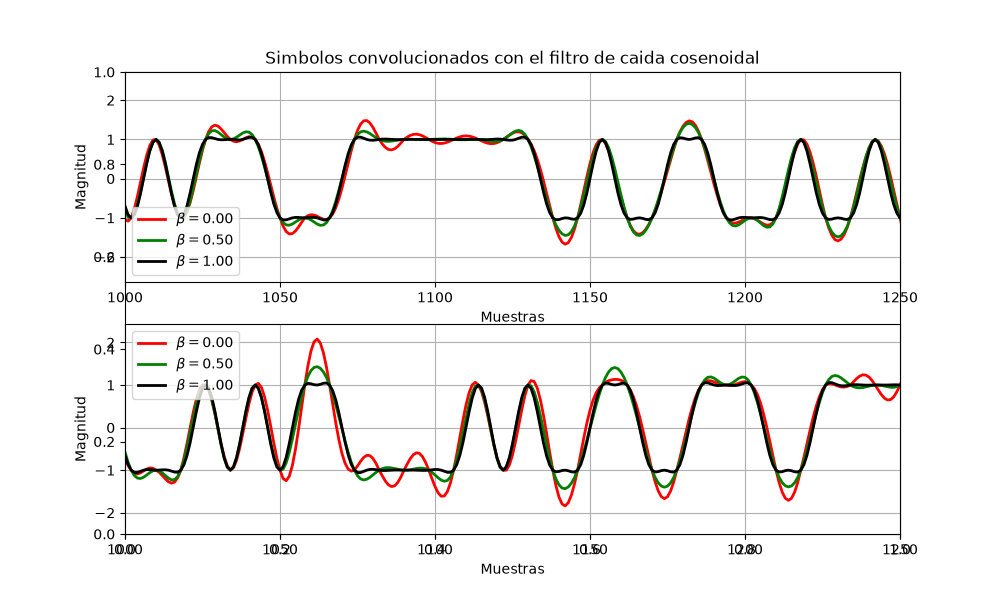
\includegraphics[width=0.85\textwidth]{../images/simbolos-filtro.png}
    \caption{Convolución de los filtros con los símbolos transmitidos en punto
        flotante.}
\end{figure}

Para observar el efecto de la cuantización, las siguientes figuras 10.a y 10.b
muestra los resultados para $\beta = 0.5$ en modo truncado y redondeado. La
cuantización $S(3,2)$ (verde) introduce distorsiones visibles en la forma de
onda, especialmente en los picos y cruces por cero. La cuantización $S(6,4)$
(azul) muestra una degradación muy leve, y $S(8,7)$ (amarillo) mantiene la
forma de onda prácticamente intacta, confirmando que con 8 bits la
representación es casi exacta.

\begin{figure}[H]
    \centering
    \begin{subfigure}[b]{0.49\textwidth}
        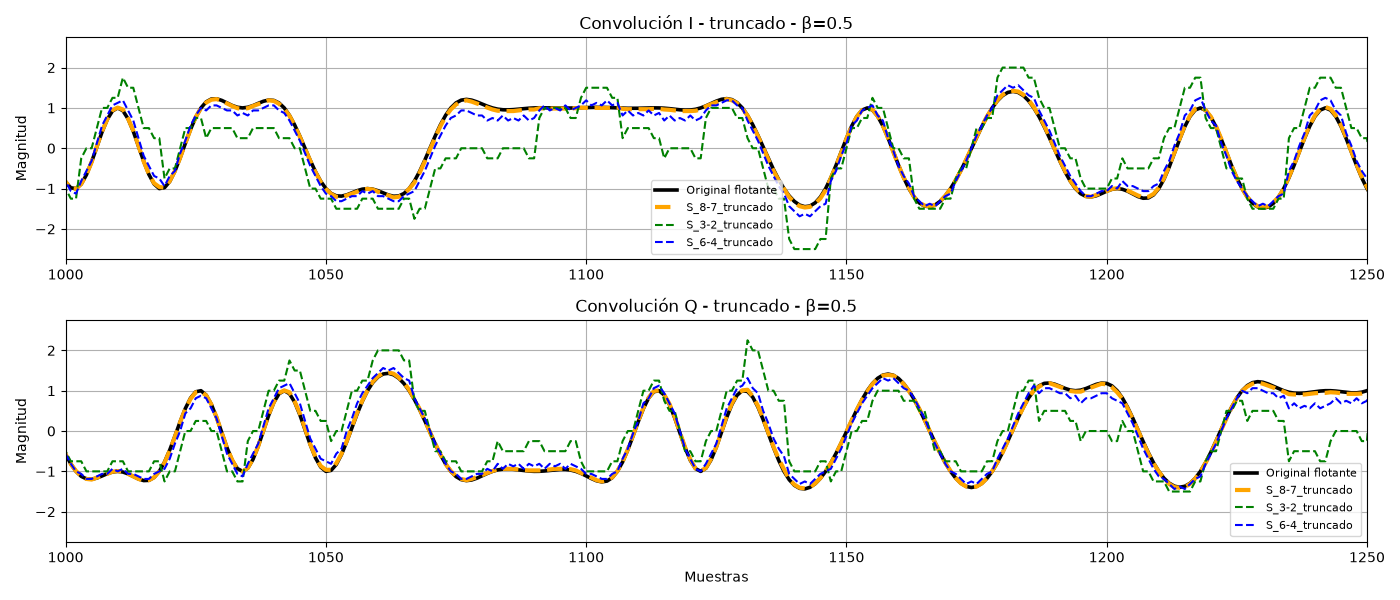
\includegraphics[width=\textwidth]{../images/cuantizaciones/convolucion_truncado_beta1.png}
        \caption{Truncado, $\beta = 0.5$.}
    \end{subfigure}
    \hfill
    \begin{subfigure}[b]{0.49\textwidth}
        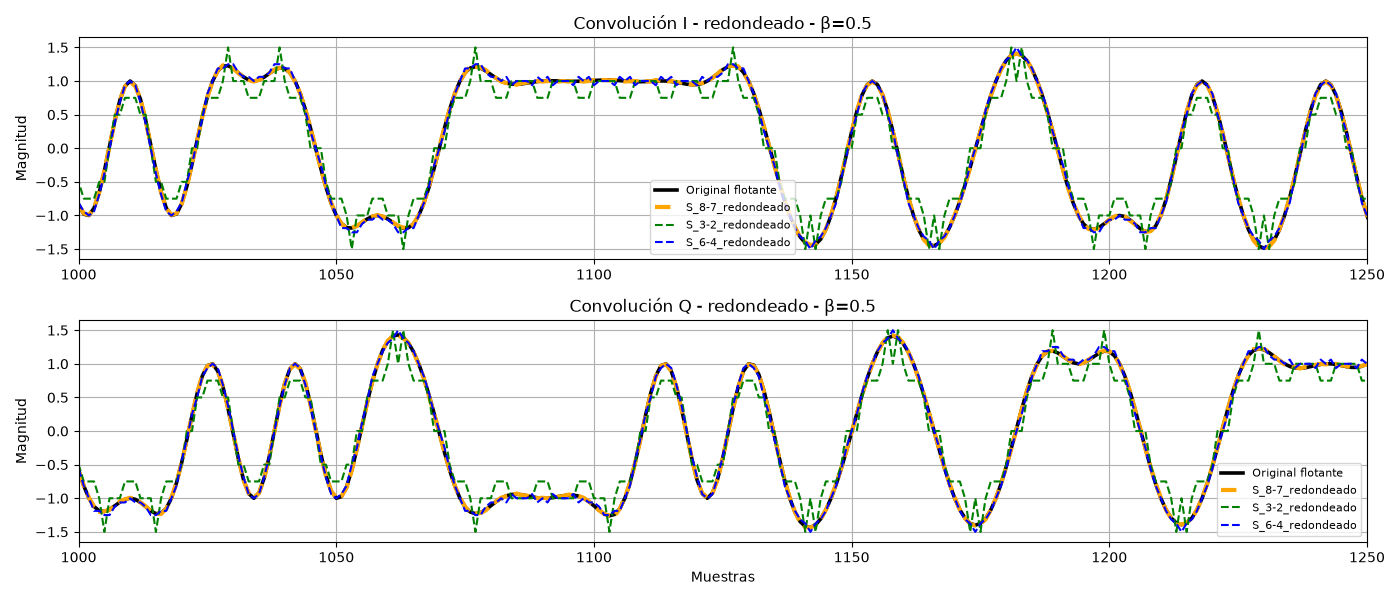
\includegraphics[width=\textwidth]{../images/cuantizaciones/convolucion_redondeado_beta1.png}
        \caption{Redondeado, $\beta = 0.5$.}
    \end{subfigure}
    \caption{Convolución cuantizada para $\beta = 0.5$.}
\end{figure}

En las Figuras 11.a y 11.b se muestran los resultados para $\beta = 0.0$ y
$\beta = 1.0$ en modo truncado y 12.a y 12.b redondeado. Se observa que $\beta
    = 0.0$ es el más afectado por la cuantización, con distorsiones notables
incluso en $S(6,4)$, mientras que $\beta = 1.0$ mantiene una forma de onda más
estable.

\begin{figure}[H]
    \centering
    \begin{subfigure}[b]{0.49\textwidth}
        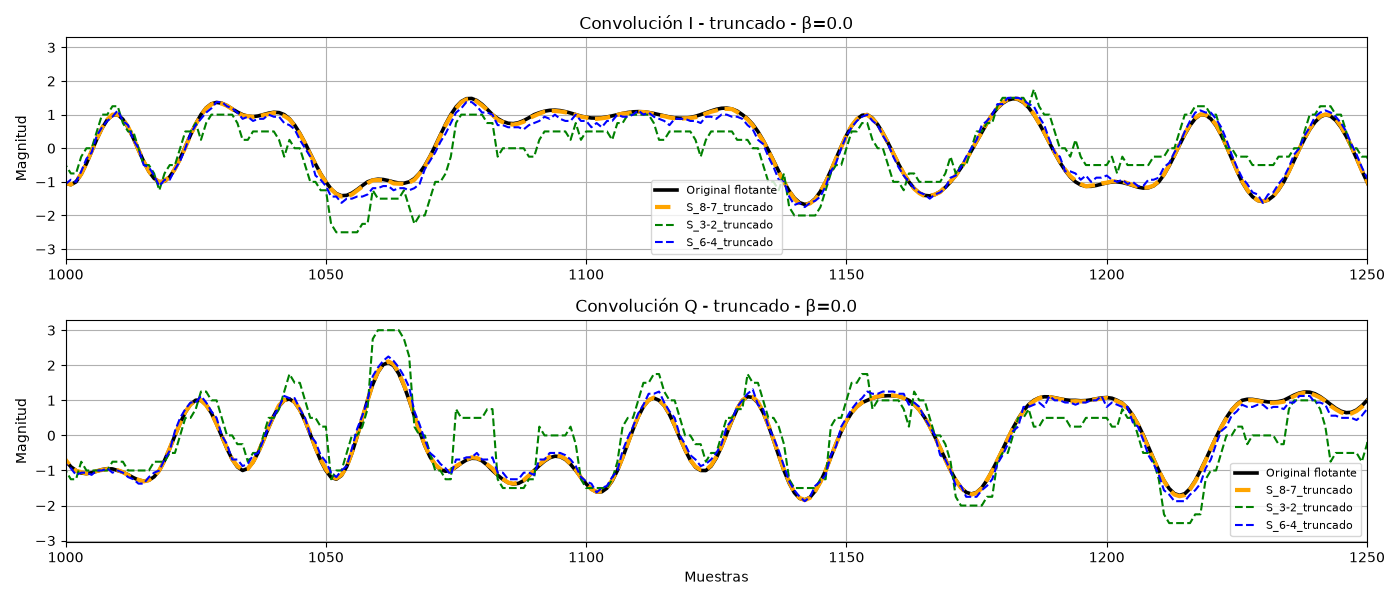
\includegraphics[width=\textwidth]{../images/cuantizaciones/convolucion_truncado_beta0.png}
        \caption{Truncado, $\beta = 0.0$.}
    \end{subfigure}
    \hfill
    \begin{subfigure}[b]{0.49\textwidth}
        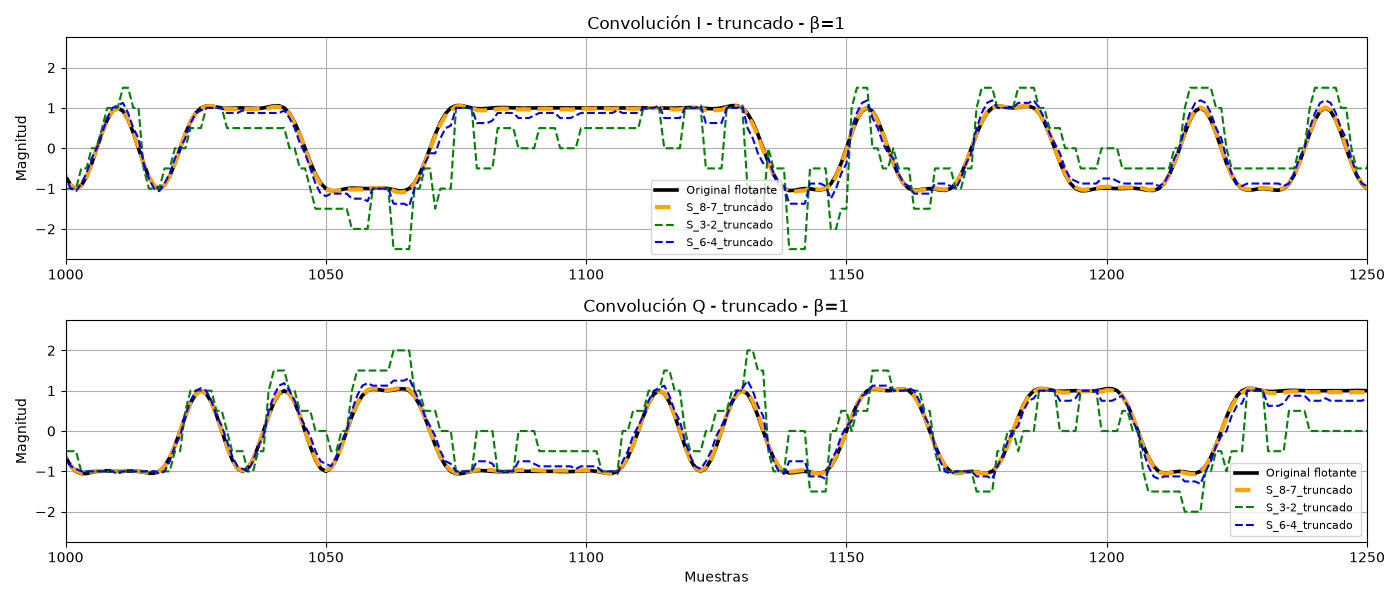
\includegraphics[width=\textwidth]{../images/cuantizaciones/convolucion_truncado_beta2.png}
        \caption{Truncado, $\beta = 1.0$.}
    \end{subfigure}
    \caption{Convolución cuantizada --- truncado.}
\end{figure}

\begin{figure}[H]
    \centering
    \begin{subfigure}[b]{0.49\textwidth}
        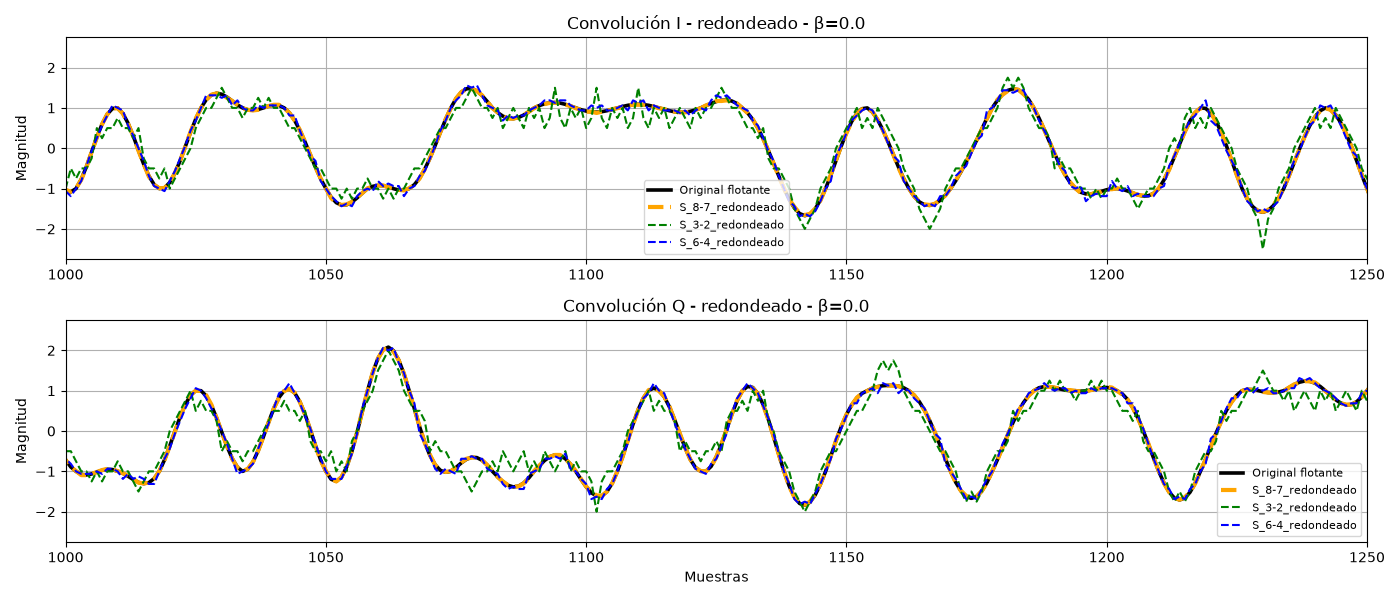
\includegraphics[width=\textwidth]{../images/cuantizaciones/convolucion_redondeado_beta0.png}
        \caption{Redondeado, $\beta = 0.0$.}
    \end{subfigure}
    \hfill
    \begin{subfigure}[b]{0.49\textwidth}
        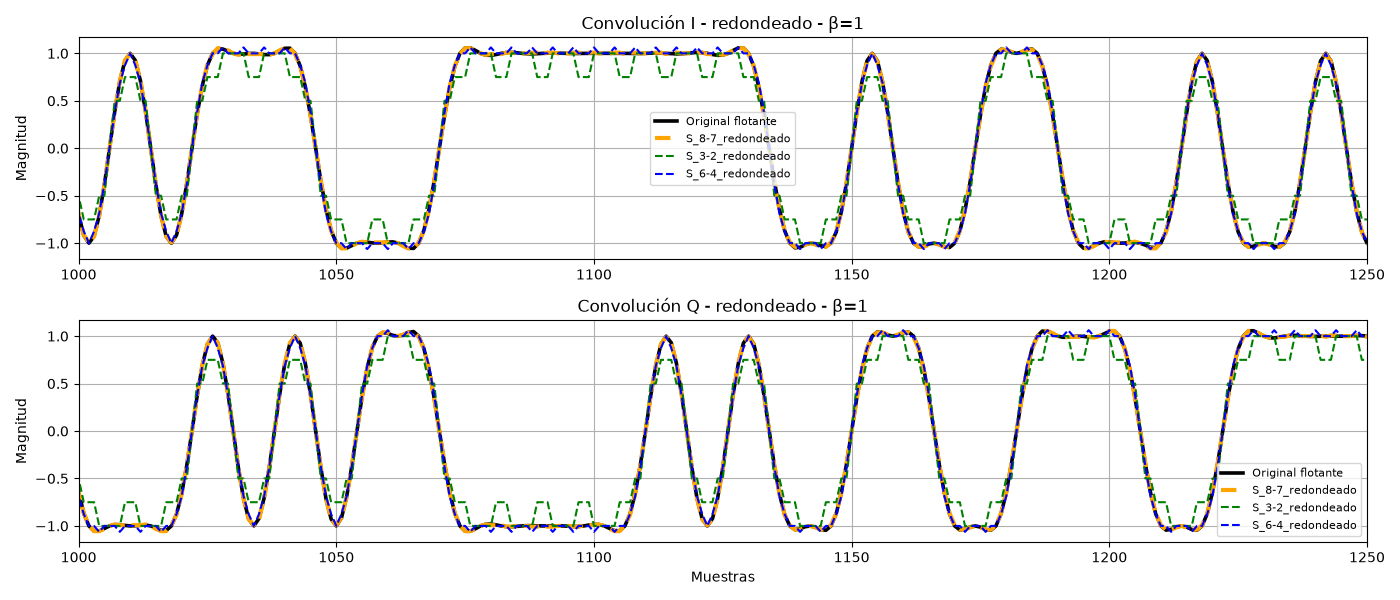
\includegraphics[width=\textwidth]{../images/cuantizaciones/convolucion_redondeado_beta2.png}
        \caption{Redondeado, $\beta = 1.0$.}
    \end{subfigure}
    \caption{Convolución cuantizada --- redondeado.}
\end{figure}

Se observa que tanto la cuantización como el roll-off afectan la forma de onda
resultante. Este efecto debe ser tenido en cuenta al momento de diseñar un
sistema de comunicaciones, ya que una forma de onda distorsionada puede
dificultar la detección de símbolos y aumentar la tasa de error de bit (BER).
Como se verá en la siguiente sección, estos efectos se vuelven más evidentes en
la constelación, donde la dispersión de los puntos en el plano I-Q refleja
directamente la pérdida de precisión introducida por la cuantización.

\subsection{Constelación}

La constelación es la representación más intuitiva del impacto de la
cuantización, ya que muestra directamente la dispersión de los símbolos
recibidos en el plano I-Q. En la Figura 13 se presenta la constelación en punto
flotante para los tres valores de $\beta$. Se observa que $\beta = 0.0$
presenta la mayor dispersión, producto de la sensibilidad del filtro sinc a la
fase de muestreo y sus colas largas. En contraste, $\beta = 1.0$ concentra los
puntos firmemente alrededor de $\pm 1$, evidenciando un filtrado más robusto.

\begin{figure}[H]
    \centering
    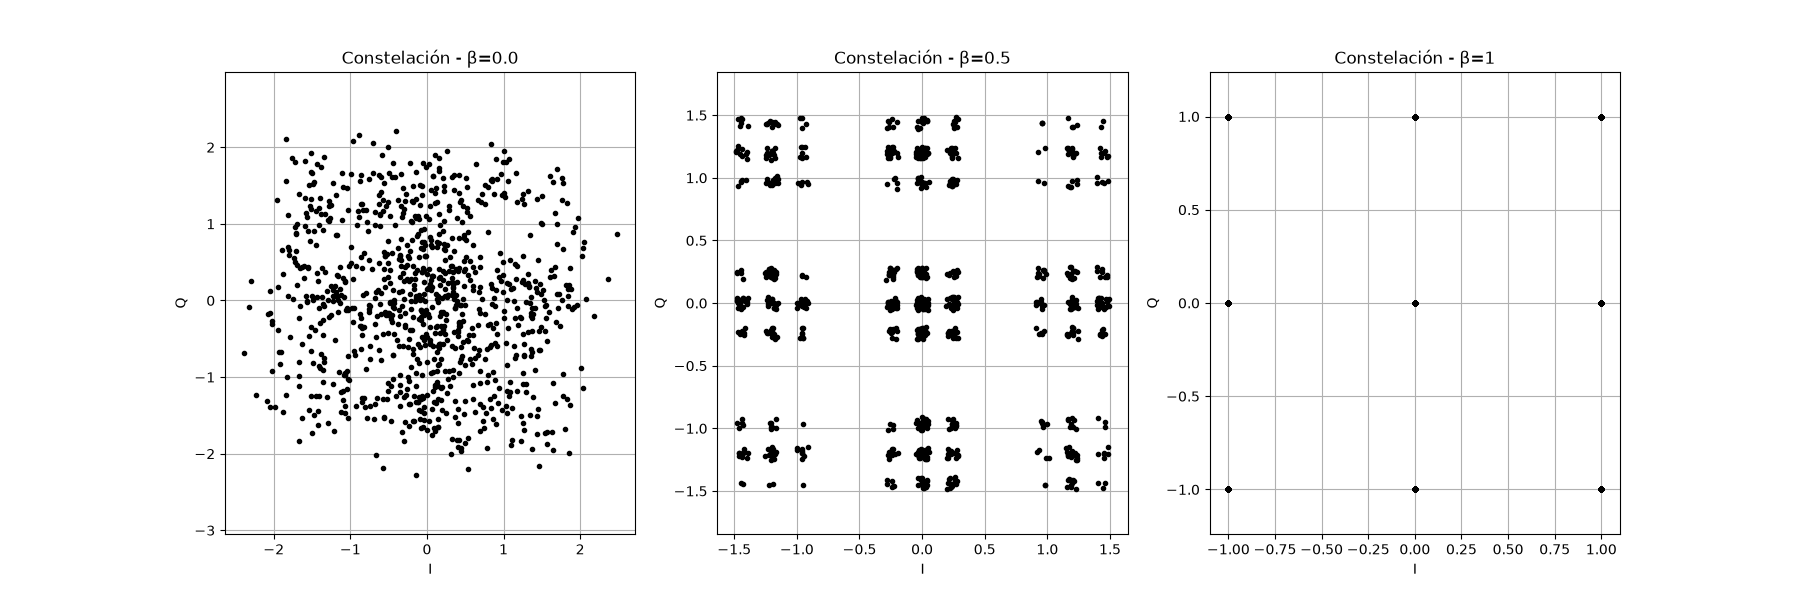
\includegraphics[width=0.85\textwidth]{../images/constelacion.png}
    \caption{Constelación de los símbolos transmitidos filtrados en punto
        flotante.}
\end{figure}

Al cuantizar los coeficientes, la constelación degrada de forma directamente
proporcional a la pérdida de resolución. En las Figuras 14.a, 14.b y 14.c se
muestran las constelaciones para las tres cuantizaciones truncadas en cada
$\beta$.

\begin{figure}[H]
    \centering
    \begin{subfigure}[b]{0.32\textwidth}
        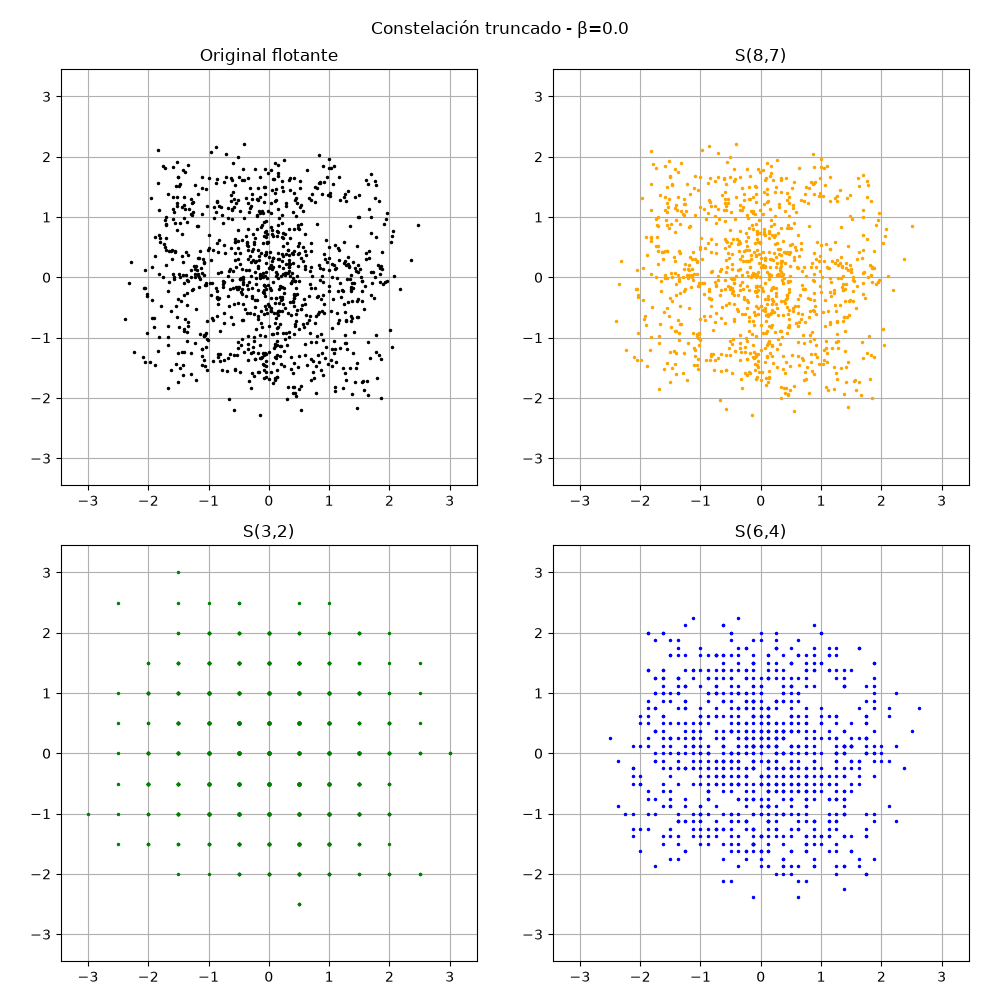
\includegraphics[width=\textwidth]{../images/cuantizaciones/constelacion_truncado_beta0.png}
        \caption{$\beta = 0.0$}
    \end{subfigure}
    \hfill
    \begin{subfigure}[b]{0.32\textwidth}
        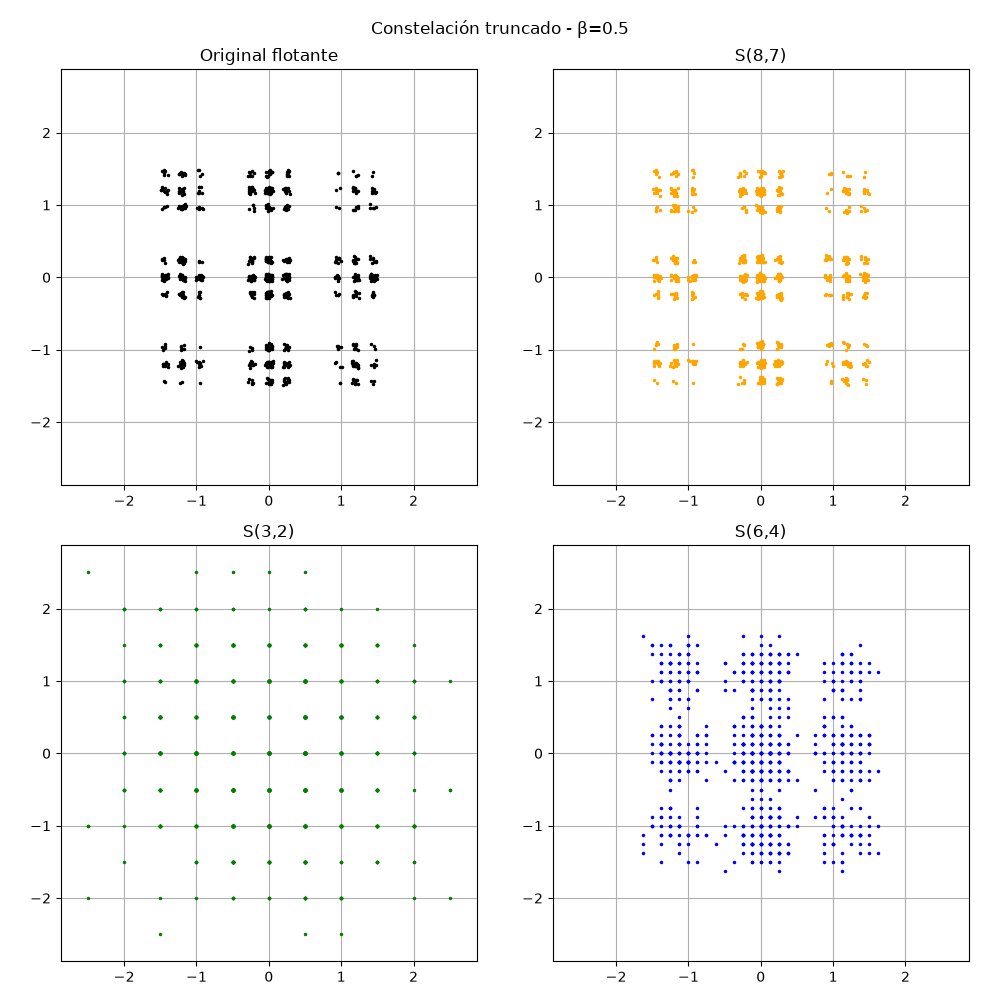
\includegraphics[width=\textwidth]{../images/cuantizaciones/constelacion_truncado_beta1.png}
        \caption{$\beta = 0.5$}
    \end{subfigure}
    \hfill
    \begin{subfigure}[b]{0.32\textwidth}
        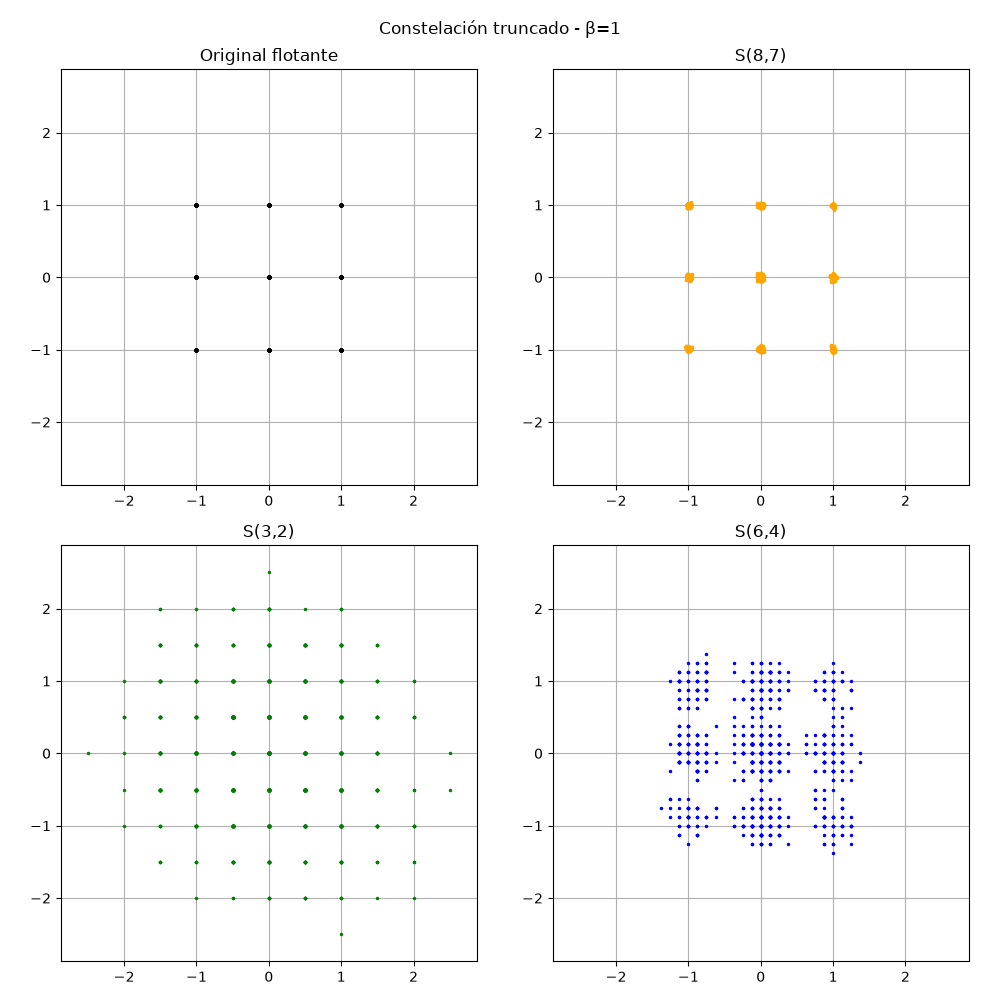
\includegraphics[width=\textwidth]{../images/cuantizaciones/constelacion_truncado_beta2.png}
        \caption{$\beta = 1.0$}
    \end{subfigure}
    \caption{Constelaciones cuantizadas --- truncado.}
\end{figure}

Los efectos varían según $\beta$:
\begin{itemize}
    \item Para $\beta = 0.0$ (izquierda) se observa una gran dispersión (incluso en el
          original flotante) y las cuantizaciones degradan aún más la constelación;
          $S(3,2)$ es prácticamente irreconocible.
    \item Para $\beta = 0.5$ (centro) la constelación presenta una dispersión intermedia,
          con $S(8,7)$ casi idéntica al original.
    \item Para $\beta = 1.0$ (derecha) todas las cuantizaciones siguen mejor la
          constelación flotante, aunque $S(3,2)$ mantiene una dispersión considerable.
\end{itemize}

En todos los casos, $S(3,2)$ presenta una estructura de niveles discretos que
evidencia la baja resolución, tomando valores multiplos de $0.5$.

En la Figura se muestran los resultados para el modo redondeado. El redondeo
produce constelaciones ligeramente más limpias que el truncado para el mismo
ancho de bits, especialmente en $S(6,4)$ y $S(3,2)$, donde distribuye el error
de forma más simétrica y evita la acumulación de bias que introduce el
truncado.

\begin{figure}[H]
    \centering
    \begin{subfigure}[b]{0.32\textwidth}
        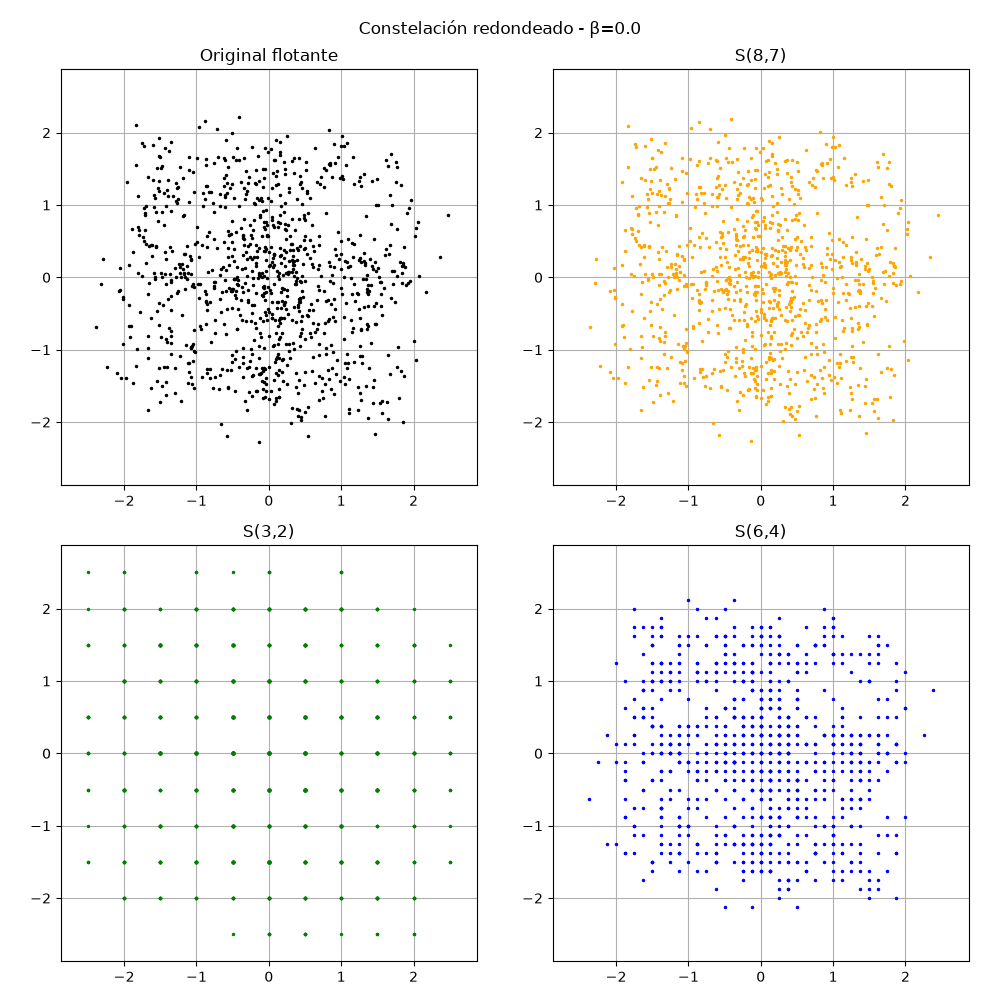
\includegraphics[width=\textwidth]{../images/cuantizaciones/constelacion_redondeado_beta0.png}
        \caption{$\beta = 0.0$}
    \end{subfigure}
    \hfill
    \begin{subfigure}[b]{0.32\textwidth}
        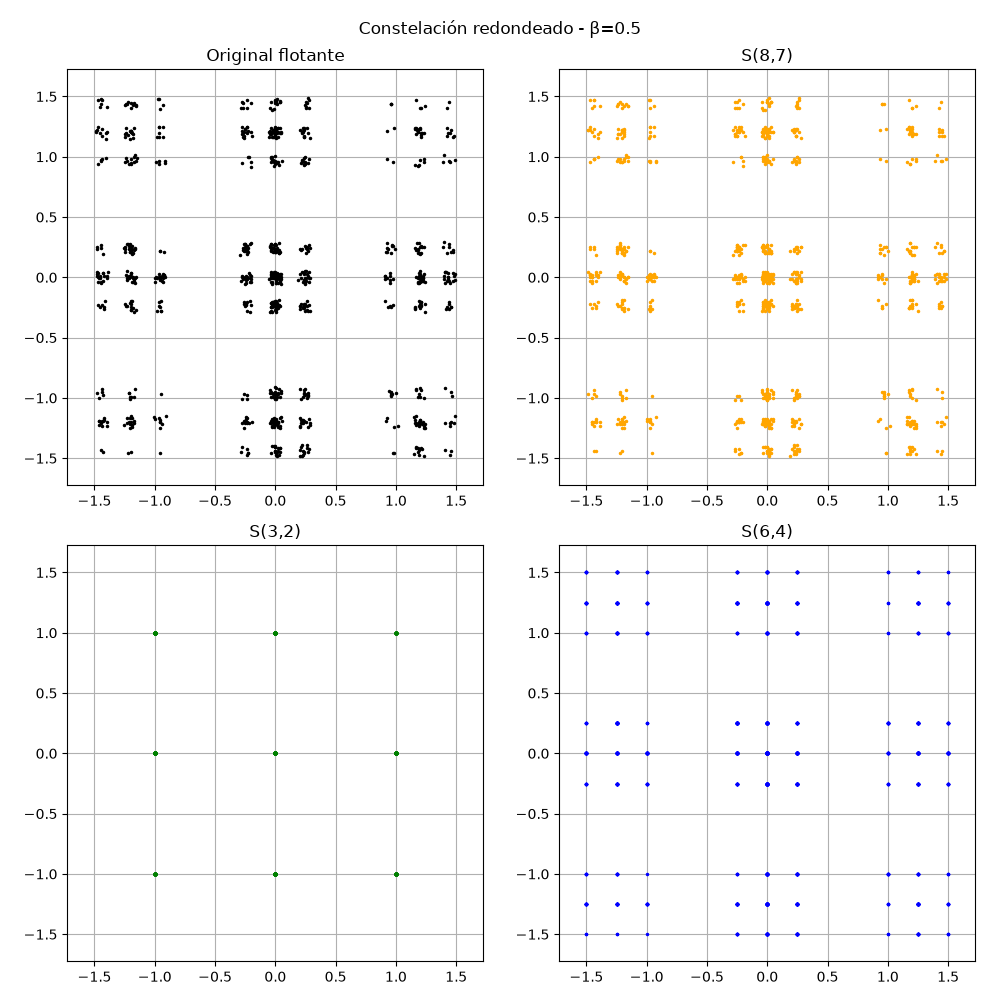
\includegraphics[width=\textwidth]{../images/cuantizaciones/constelacion_redondeado_beta1.png}
        \caption{$\beta = 0.5$}
    \end{subfigure}
    \hfill
    \begin{subfigure}[b]{0.32\textwidth}
        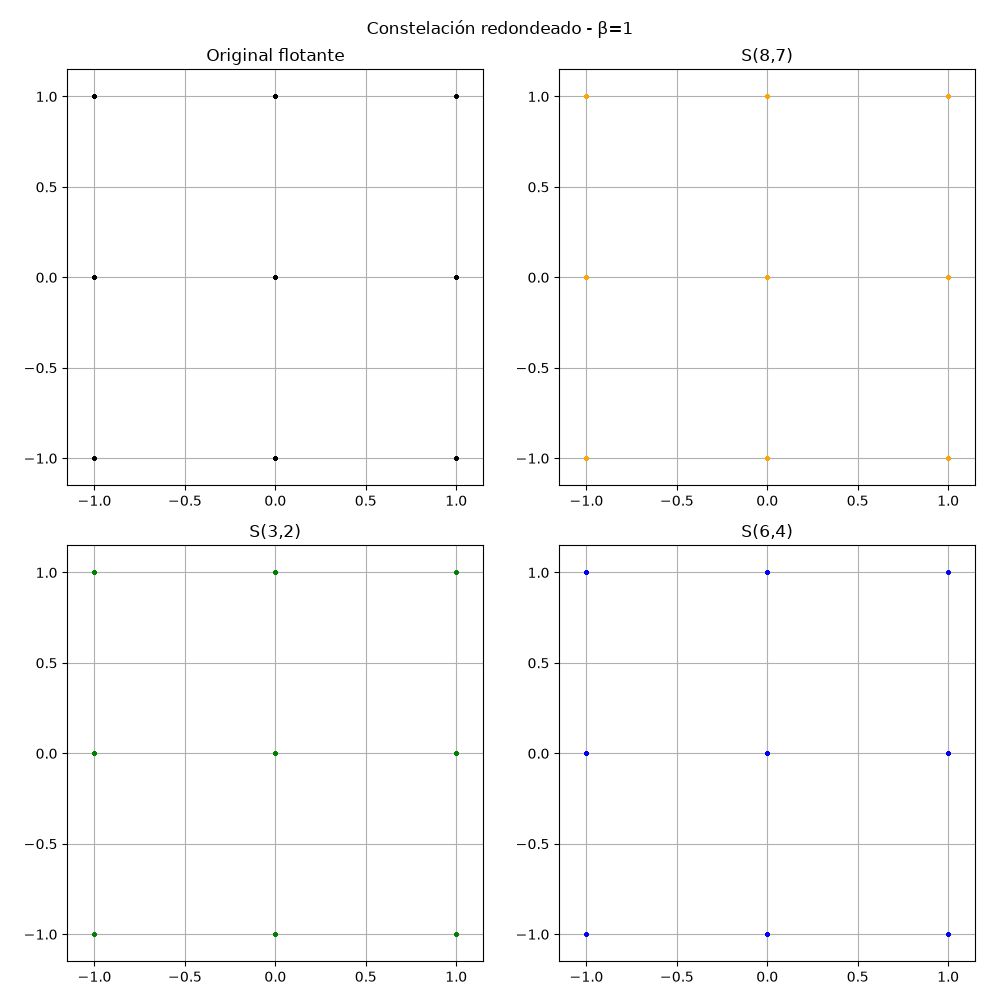
\includegraphics[width=\textwidth]{../images/cuantizaciones/constelacion_redondeado_beta2.png}
        \caption{$\beta = 1.0$}
    \end{subfigure}
    \caption{Constelaciones cuantizadas --- redondeado.}
\end{figure}

\section{Conclusiones}

A partir de los resultados obtenidos, se pueden extraer las siguientes
conclusiones:

\begin{itemize}
    \item La cuantización $S(8,7)$ (\texttt{trunc} y \texttt{round}) produce resultados
          prácticamente idénticos al punto flotante en todas las métricas evaluadas,
          siendo una opción adecuada cuando se requiere alta fidelidad con un costo de
          hardware moderado.

    \item La cuantización $S(6,4)$ introduce errores visibles pero aceptables en
          aplicaciones no críticas. El efecto es más notorio en el piso de ruido de la
          respuesta en frecuencia y en la dispersión de la constelación.

    \item La cuantización $S(3,2)$ degrada severamente el rendimiento del sistema. La
          resolución de $0.25$ es insuficiente para representar adecuadamente los
          coeficientes del filtro, resultando en una constelación con solo 4 niveles por
          eje y una respuesta en frecuencia con un piso de ruido elevado.

    \item El modo \texttt{round} ofrece mejores resultados que \texttt{trunc} para el
          mismo ancho de bits, siendo recomendable su uso cuando el hardware lo soporte.

    \item El filtro con $\beta = 1.0$ es notablemente más robusto a la cuantización que
          $\beta = 0.0$, debido a que sus coeficientes tienen una dinámica más acotada y
          colas que decaen más rápidamente.
\end{itemize}

\end{document}